\section{Introduction}
\label{sec:intro}

An {\em ad hoc data format} is any nonstandard data format for which
parsing, querying, analysis or transformation tools are not readily
available.  \xml{} is not an ad hoc data format --- there are hundreds
of tools for reading, querying, and transforming \xml{}.  However,
computer programmers, financial analysts, computational biologists,
chemists and physicists, healthcare and airline information systems,
corporate IT professionals and others deal with deal ad hoc data in a
myriad of complex formats on a daily basis.  This data is often
unpredictable, poorly documented, and filled with errors, making it
extremely difficult to deal with.  Often, before anything can be done
with ad hoc data one must clense it of as many errors as possible,
normalize its shape and transform it into a standardized format.  Once
in a standardized format, the data can be directly loaded into a
database or manipulated by standard, widely available tools.

% The goal of this paper is to describe a new language for efficient and
% reliable computing with ad hoc data.  More specifically, we describe a
% high-level programming language, \datatype{}, that comes with
% intrinsic support for processing ad hoc data.  Our programming
% language will use the rich data descriptions both as directives for
% parsing ad hoc data sources and as types for describing
% representations of ad hoc data within the programming environment.  In
% addition, a critical facet of our language will be its support for
% {\em error-aware computing}.  Our error-aware infrastructure will
% allow programmers to conveniently verify correctness of data relative
% to a description or alternatively detect data errors and handle them
% in domain-specific ways.  Finally, we will be sure our language design
% is founded on strong programming language principles by studying its
% type system and metatheory extensively.

There are vast amounts of useful data stored in traditional databases
and \xml{} formats, but there is just as much in ad hoc formats.
\figref{figure:data-sources} provides some information on ad hoc data
formats from the networking and telecommunications domain at AT\&T and
ad hoc data formats used by computational biologists at Princeton.
They include ASCII, binary, and Cobol data formats, with both fixed
and variable-width records arraged in linear sequences or in tree- or
DAG-shaped hierarchies.  The data sources range in size from
relatively small files up to network applications, such as web server
logs, which can be produced at a rate of 12GB per week, to Netflow
applications, which can be produced at over one GB per second.  Common
errors include undocumented data, corrupted data, missing data, and
multiple missing-value representations.

We hope that these examples give the reader a beginning sense of the
nature and pervasiveness of ad hoc data sources.  However, we cannot
emphasize enough just how pervasive ad hoc data is and to what degree
it infiltrates computer systems, businesses, government, and
scientific research.  Remember, just about any program that spits out
useful information in a format other than \xml{}, \textsc{html},
\textsc{jpeg}, \textsc{mpeg} or a few others is generating ad hoc
data.  Hence, most programmers deal with ad hoc data on a individual
basis regularly.  When it comes to ad hoc data on a grand scale,
perhaps the most daunting challenge will come from the national
health-care system.  Recently, Newt Gingrich and Hilary Clinton have
jointly proposed we consolidate and integrate our national healthcare
records in the next 10 years.  Such a massive project will undoubtedly
require technical solutions at many levels.  At the lowest levels, we
will need a reliable software to collect and transfer health care data
from legacy systems into modern formats.  The \datatype{} system we
propose will be an invaluable aid in the development of this software.

\begin{figure*}
\begin{center}
\begin{tabular}{@{}|l|l|l|l|}
\hline
Name: Use                           & Representation    
%& Size
           & Common Errors \\ \hline\hline
Web server logs (CLF):                & Fixed-column      
%& $\leq$12GB/week 
& Race conditions on log entry\\ 
Measuring web workloads               & ASCII records     
%&                             
& Unexpected values\\ \hline
AT\&T provisioning data (\dibbler{}): & Variable-width    
%& 2.2GB/week 
& Unexpected values \\ 
Monitoring service activation         & ASCII records     
%&            
& Corrupted data feeds \\ \hline
Call detail:                   & Fixed-width       
%&\appr{}7GB/day 
&  Undocumented data\\
Fraud detection 
                                      & binary records  
%& 
& \\ \hline 
AT\&T billing data (\ningaui{}):      & Cobol  
%& \appr{}4000 files/day, 
& Unexpected values\\ 
Monitoring billing process   &                             
%& 250-300GB/day    
& Corrupted data feeds \\ \hline
IP backbone data (\darkstar{})  & ASCII  
%& $\ge$ 15 sources  
& Multiple missing-value rep's \\
Network Monitoring:  &        
%& \appr{}15 GB/day              
& Undocumented data \\ \hline
Netflow                               & Data-dependent      
%& $\ge$1Gigabit/second  
& Missed packets\\ 
Network Monitoring:        & number of   
%&                       
& \\
                                      & fixed-width 
%&
& \\
                                      & binary records 
%&
& \\ \hline
Gene Ontology data:        & Variable-width ASCII records 
%& ? 
&  \\
Gene-gene correlations in Magic & in DAG-shaped hiearchy 
%&  
& \\
database &
%& 
& \\\hline
Newick data                          & Fixed-width ASCII record 
%& ? 
& Manual entry errors \\
Immune system response simulation & in tree-shaped hierarchy 
%& 
& \\
\hline
\end{tabular}
\caption{Selected ad hoc data sources.}
\label{figure:data-sources}
\end{center}
\end{figure*}

Processing all this ad hoc data is challenging for a variety of
reasons.  First, ad hoc data typically arrives ``as is'': the analyst
or system that receives it can only say ``thank you,'' not request a
more convenient format.  Second, documentation for the format may not
exist at all, or it may be out of date.  A common phenomenon is for a
field in a data source to fall into disuse.  After a while, a new
piece of information becomes interesting, but compatibility issues
prevent data suppliers from modifying the shape of their data, so
instead they hijack the unused field, often failing to update the
documentation in the process.

Third, such data frequently contain errors for a variety of reasons:
malfunctioning equipment, race conditions on log entry~\cite{wpp},
non-standard values to indicate ``no data available,'' human error in
entering data, unexpected data values, \etc{} The appropriate response
to such errors depends on the application.  Some applications require
the data to be error free: if an error is detected, processing needs
to stop immediately and a human must be alerted.  Other applications
can repair the data, while still others either set data aside for a
human user to investigate or simply discard the erroneous or
unexpected values altogether.  For some applications, errors in the
data can be the most interesting part because they can signal where
two systems are failing to communicate.

A fourth challenge is that ad hoc data sources can be high volume:
AT\&T's call-detail stream contains roughly 300~million calls per day
requiring approximately 7GBs of storage space. Although this data is
eventually archived in a database, analysts mine it profitably before
such archiving~\cite{kdd98,kdd99}. More challenging, the \ningaui{}
project at AT\&T accumulates billing data at a rate of 250-300GB/day,
with occasional spurts of 750GBs/day. Netflow data arrives from Cisco
routers at rates over a gigabyte per second~\cite{gigascope}! Such
volumes mean it must be possible to process the data without loading
it all into memory at once.

A final challenge is that ad hoc data often needs to be translated
into a new, more useful or more standard format before anything can be
done with it.  Intuitively, this transformation can be done in three
stages.  First, one must generate a parser for the ad hoc format to
read it into a program.  Second, one must engineer the transformation
itself by filtering unwanted parts, normalizing representations, and
detecting and correcting or deleting erroneous data.  Third,
transformed data must be printed in the new format that can be
processed by standards tools.

Today, people tend to use \C{} or \perl{} for this task.
Unfortunately, writing parsers, transformations and printers this way
is tedious and error-prone, complicated by the lack of documentation,
convoluted encodings designed to save space, the need to produce
efficient code, and the need to handle errors robustly to avoid
corrupting down-stream data.  Moreover, the parser writers' hard-won
understanding of the data ends up embedded in parsing code, making
long-term maintenance difficult for the original writers and sharing
the knowledge with others nearly impossible.

Solution: Data description Language + transform language
Combine data description language with a transform language.
\pads{} is bound to C. However, functional programming languages are
better suited to the task of data tranformation. We therefore propose
a new language, \datatype{}, that combines a data description language
based on the style of ML types (and datatypes) with a functional data
transformation language. 

Our contributions are twofold. First, we propose an ML-style syntax
for the \pads{} data description language, based on type definitions
and {\em(polymorphic coming soon?)} parameterized recursive datatypes
(support for recursive datatypes is new to the \pads{} language, based
on recent results in our other work). This new syntax has a number of
advantages. It is more concise than the C-style encoding and more
naturally suited to describing recursive datatypes. Most importantly,
the new syntax is much more appropriate for transformation language
proposed below, which is based heavily on pattern-matching and data
constructors.

Our second contribution is the data transformation language itself.
{\em \pads{} is not a programming language.}  It merely generates
libraries that can be used by \C{} programmers.  \C{} is a very
low-level language that makes transforming ad hoc data awkward,
cumbersome and potentially error-prone.  More importantly, it provides
no intrinsic support for dealing with the errors that appear in ad hoc
data.  In addition, \C's type system and operational model provide no
support for checking the rich invariants found in ad hoc data either
at run time or at compile time.  In contrast, \datatype{} is a
high-level language with an elegant and convenient syntax for
data-driven programming, intrinsic support for handling errors and
intrinsic mechanisms for checking data invariants at run time {\em
  coming soon: and a sophisticated type system for enforcing data
  invariants at compile time}. 

At its core, \datatype{} is a functional language with standard
features such as pattern matching and higher-order functions, which we
view as critical to supporting data-driven transforms. In addition,
\datatype{} allows programmers to enforce semantic constraints on
data by using \datatype{} descriptions as a special form of runtime
contracts. The basic values of the language will be pairs of data
items and their corresponding meta-data. For each data item, the meta
data will include, among other things, descriptions of the error
content of the data item. Through the type system, the language will
ensure that data and associated meta data are kept in sync. This
property (which we call ``error-aware computing'') enables three
critical language features.
\begin{enumerate}
\item Safe, error-transparent transformations
\item Error querying - analyst can extract detailed picture of data
  error profile.
\item Flexible, programmatic repair of faulty records - analyst can
  choose when in the processing stream to address errors, rather than
  being forced to drop all faulty records at the beginning of the process.
\end{enumerate}

In the next section, we will describe, in detail, the \pads{} approach
to data and meta data (inherited by \datatype{}), the \datatype{}
syntax for data description, and illustrative examples. Next, in
section~\ref{sec:data-transformation} we will elaborate on
\datatype{}'s support for data transformation, including design,
syntax, brief overview of the semantics and some examples.
Section~\ref{sec:implementation-techniques} will discuss our proposed
implementation techiniques, and section~\ref{sec:related-work} the
related work. A discussion of conclusions and future work is included
in section~\ref{sec:conclusion}.


\subsection{Architecture}

\begin{figure}[tp]
  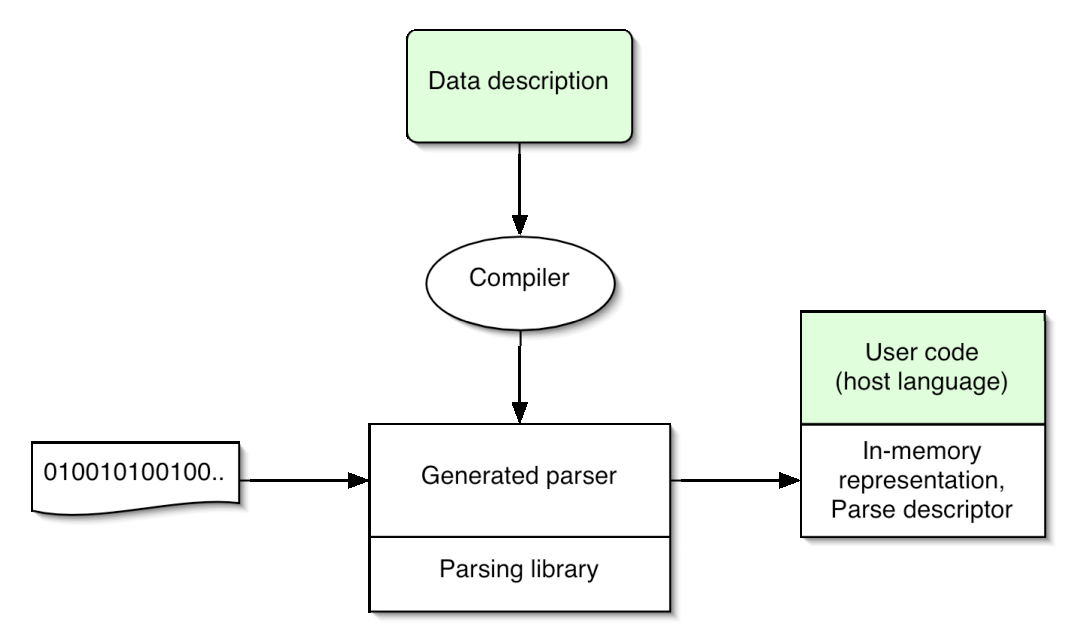
\includegraphics[height=3in,width=5in]{architecture.eps}
%  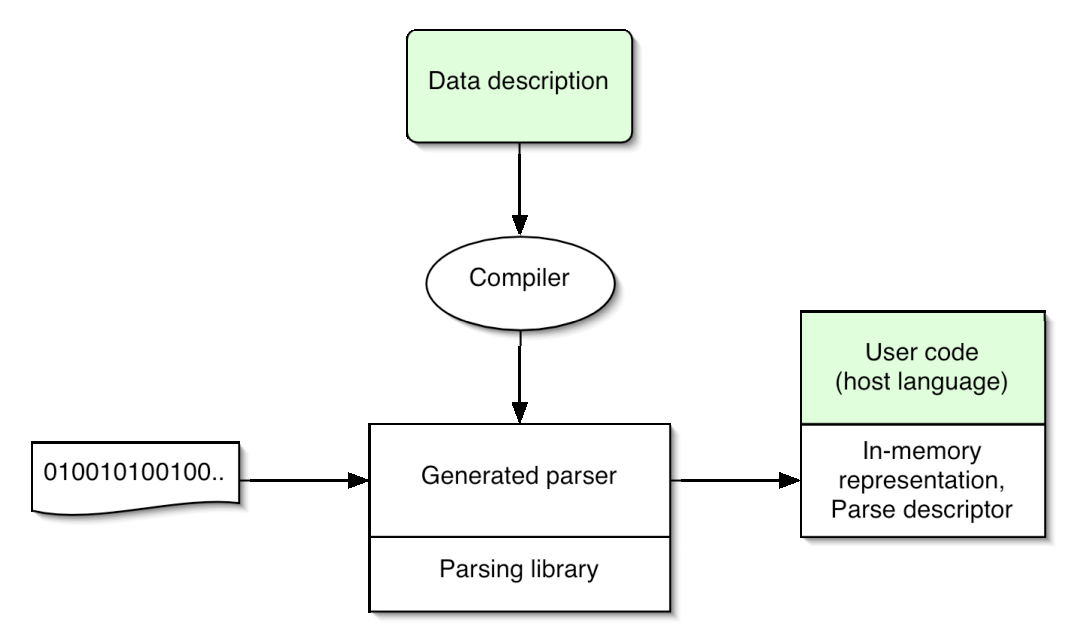
\includegraphics{architecture.eps}
\label{fig:pads-arch}
\caption{The \pads{} Architecture}
\end{figure}
